215. \begin{figure}[ht!]
\center{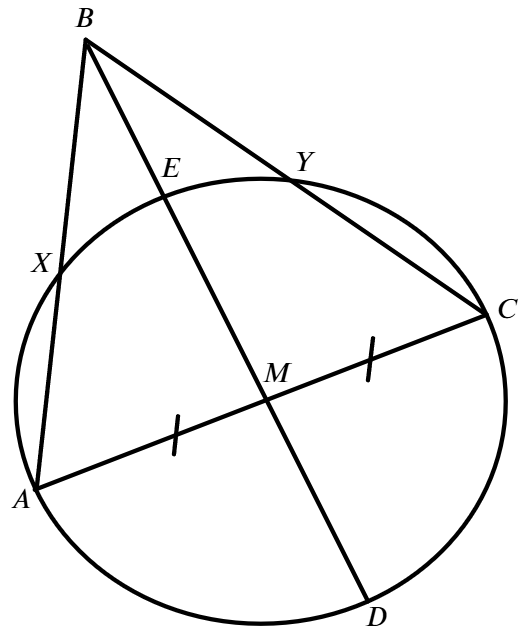
\includegraphics[scale=0.35]{g9-210.png}}
\end{figure}\\
По свойству отрезков секущей имеем равенство $BX\cdot BA=BE\cdot BD=(BM-10)(BM+10)=BM^2-100,\ BX=\cfrac{BM^2-100}{BA}.$ По формуле для медианы треугольника $ABC$ получим соотношение: $BX=\cfrac{BM^2-100}{BA}=\cfrac{\cfrac{2BA^2+2BC^2-AC^2}{4}-100}{BA}
=\cfrac{2BA^2+2BC^2-800}{4BA},$ тогда $AX=BA-BX=BA-\cfrac{2BA^2+2BC^2-800}{4BA}=\cfrac{2BA^2-2BC^2+800}{4BA}.$ Аналогично верно и равенство
$CY=\cfrac{2BC^2-2BA^2+800}{4BC},$ таким образом $AX\cdot AB+CY\cdot BC=\cfrac{2BA^2-2BC^2+800}{4}+\cfrac{2BC^2-2BA^2+800}{4}=\cfrac{800+800}{4}=400\text{ см}^2.$
\end{document}